%----------------------------------------------------------------------------
\chapter{Model-based testing}
\label{cha:modelbasedtesting}
%----------------------------------------------------------------------------

The idea of model-based testing originates from the 70's, and now it has an extensive literature, terminology and a commonly accepted taxonomy \cite{taxonomy}. This section introduces the concept of this variant of software testing through a concrete process (Figure~\ref{fig:mbtprocess}).

\begin{figure}[htp]
\centering
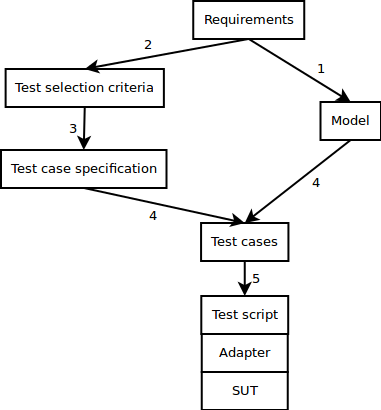
\includegraphics[scale=0.6]{figures/mbt_process.png}
\caption{Model-based testing process}
\label{fig:mbtprocess}
\end{figure}

\begin{enumerate}
    \item From informal requirements or created specifications a model can be built. The model is an abstract representation of the \textit{system under test (SUT)}. It uses encapsulation for information reduction, because it has to be more simple, than the original system to achieve an easier modifying and maintaining \cite{mbttestcasegeneration}. During a model-based software development the model can be used for many other tasks too, as it serves analysing, synthesising and documenting the SUT as well.
     \item Test selection criteria decide how the test cases are chosen, which point of view is important by testing. These selected criteria will control the whole test generation process.
     \item Criteria are transformed into \textit{test case specifications}. These test case specifications are the formalised versions of the criteria.
     \item After creating the model and the test case specifications set of \textit{test cases} is generated from the model regarding all the specifications. One of the biggest challenges is to create the test cases. A simple test case consists of a pair of input parameters and expected outputs. Finite set of test cases forms a \textit{test suite}. The difficulty comes from the need to satisfy the test case specifications and create a minimised set of test cases.
     \item A successfully generated test suite can be executed on the SUT. For the execution a \textit{test script} can be used, which executes the test cases.
     
     The generated test cases are strongly linked to the abstract test model, therefore an \textit{adaptor} component is needed, which is often part of the test script. The adaptor adapts the test inputs to the SUT. For example if the input of a method is an XML document containing an integer value, the adaptor has to transform the test case's test inputs to XML.
     
     The test script also contains usually a \textit{test oracle}, that checks the test output difference from the expected output.
\end{enumerate}

\section{Taxonomy}
\label{sec:taxonomy}

Utting, Pretschner and Legeard investigated the currently available MBT solutions and defined (Figure~\ref{fig:mbttaxonomy}) a taxonomy which concentrates to three major properties of model-based testing. The three dimensions of their taxonomy are the modelling specification, test generation and test execution.

\begin{figure}[htp]
\centering
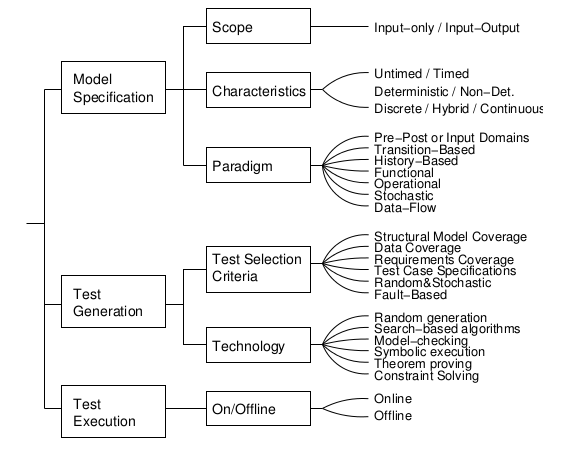
\includegraphics[scale=0.5]{figures/mbt_taxonomy.png}
\caption{Model-based testing taxonomy \cite{taxonomy}}
\label{fig:mbttaxonomy}
\end{figure}

\begin{description}
	\item[Model scope] The scope of the modelling is a binary decision. The model either specify \textit{just the test input} or \textit{the input-output pairs} for the SUT. The first case is less useful, because the test script can not check the SUT's output and that's why it is impossible to create an oracle that way.
	
	\item[Model characteristics] The SUT assigns the main characteristics of the model. It depends on the SUT's timing properties (\textit{timed} / \textit{untimed}), determinism (\textit{deterministic} / \textit{non-deterministic}) and dynamics (\textit{discrete} / \textit{continuous} / \textit{hybrid}).
	
	\item[Model paradigm] The third dimension is the paradigm that is used to describe the model. \textit{State-based notation} means, that set of variables defines the model, which represents the internal state of the system and there are some operations that modify those variables. Usually these operations given by preconditions and postconditions. By \textit{transition-based notation} the model focuses on the transition between the state of the system. Finite state machines are examples of this paradigm. \textit{History-based notations} model the allowable traces of its behaviour over time. By \textit{functional notation} collection of mathematical functions model the system. \textit{Operational notations} describe the model as a set of executable processes running parallel. Petri nets are good forms of this notation. \textit{Stochastic notations} describe the model by a probabilistic model, so it is rather suitable to model the environment than the SUT itself. An example can be the Markov chains for this type of model paradigm. The last paradigm is the \textit{data-flow notation}, where the main concept is the concentration to the data, rather than the control flow, example can be the often used Matlab Simulink model.
	
	\item[Test selection criteria] Test selection criteria control the test case generation. \textit{Structural model coverage criteria} aim to cover a part of the model, for example nodes and arcs of the transition-based model. The nodes of such a model represent the states of the system, and the arcs represent the transitions respectively. The basic idea of \textit{data coverage criteria} is to split the data space to equivalence classes and choose values from them. \textit{Requirements based coverage criteria} are linked to the informal requirements of the SUT and it applies the coverage to the requirements. \textit{Ad-hoc test case specifications} guides by the test case specifications. \textit{Random and stochastic criteria} are useful rather to model the environment and applicable to use with a stochastic model. \textit{Fault-based criteria} can be very efficient, because it concentrates to error finding in the SUT.
	
	\item[Test generation technology] One of the most important thing that defines the test case generation is the chosen technology. The easiest one to implement is the \textit{random generation}, more difficult are the \textit{search-based algorithms} where graph algorithms and other search algorithms are used to perform a walk on the model. \textit{Model checking} can also be used for test case generation, where the model checker searches for a counter-example, which becomes a test case. \textit{Symbolic execution} means analysing the software to determine what inputs cause each part of a program to execute. This method guided by test case specification to reach a goal, and test inputs become inputs which produce different outputs. \textit{Deductive theorem proving} is similar to model checking, but the model checker is replaced with a theorem prover. \textit{Constraint solving} is useful for selecting data values from complex data domains.
	
	\item[Test execution] The tests can run either \textit{online} or \textit{offline} on the SUT. During an online test, the test generator can respond to the SUT's actual output for example with an different test case sequence. By an offline test generation test cases are generated strictly before the execution.
	
	The testing can be started by an automatic execution or manually, that triggers the user directly.
\end{description}

% section taxonomy (end)

\section{Process}
\label{sec:process}

\subsection{Modelling}
\label{sub:modelling}

The first step of the model based testing process is to create a suitable model, from which a test suite can be generated. As we earlier saw by the taxonomy section \cite{sec:taxonomy}, all the identified model paradigms used in model based testing belong to some kind of behaviour modelling notation. This is not a surprise, because a data or functional model can not be utilised so effectively by software testing. Each model paradigm concentrates on a different aspect of the behaviour.

There is a plethora of technologies for modelling behaviour, and one of the most frequently used are the extended finite state machine (EFSM) and all of its variations. These variations mostly use transition based notation, but they can combine it with other modelling paradigms as well. The second most popular modelling language is the UML language, which is an enhanced version of EFSMs. Other modelling languages are used in the field of MBT too, but mostly these tools made for a specific purpose.

As EFSMs or at least their variations serve as basic modelling notation for the most available model based testing tools, that's why we have to investigate them properly. The basic parts of the UML language will be described here as well.

\subsubsection{Extended finite state machines}
\label{ssub:efsm}

A \textit{finite state machine} is a 6-tuple $\langle S, I, A, R, \Delta, T\rangle$, where
\begin{align*}
& S: \text{set of finite states},\\
& I \subset S: \text{set of initial states},\\
& A: \text{finite alphabet of input symbols},\\
& R: \text{set of possible outputs},\\
& \Delta \subset S \times A: \text{set of possible input relations},\\
& T: \text{is a transition relation function}\ f: \Delta \rightarrow S \times R
\end{align*}

The semantic of this model is the following. When $T(s, a) = (s', r)$, the state machine is receiving an input $a \in A$, when in state $s \in S$, assuming $(s,a) \in \Delta$, then the system moves to the new state $s' \in S$, and outputs $r \in R$. A possible $(s'', a') \notin \Delta$ is interpreted as an input symbol, that is not allowed in that state.

An \textit{extended finite state machine} differs from a simple finite state machine in terms of the states defined differently. The states of an extended state machine has the form $S = D_0 \times D_1 \times \dots D_n$, where $D_0$ is the set of control states, and $D_{i=1}^n$ is the domain of state variables $x_i$, that are assigned to each states.

% subsubsection efsm (end)

\subsubsection{UML state machines}
\label{ssub:umlstatemachine}

UML state machines or UML state charts are improved versions of the mathematical concept of finite state machines expressed with the OMG's Unified Modeling Language. The original state machine model suffer greatly by the state and transition explosion problem, because the complexity of these models tend to grow faster as the modelled system. UML state machines solved this problem by eliminating the common parts of these system and sharing the common behaviour across the states.

The behind idea behind the notation is, that an entity or each of its sub-entities is always in exactly one of the possible states and there are well-defined conditional transitions between these states. There are two kinds of state machine, which can be used to define behaviour of model elements or describe protocol usage.

\begin{figure}[htp]
\centering
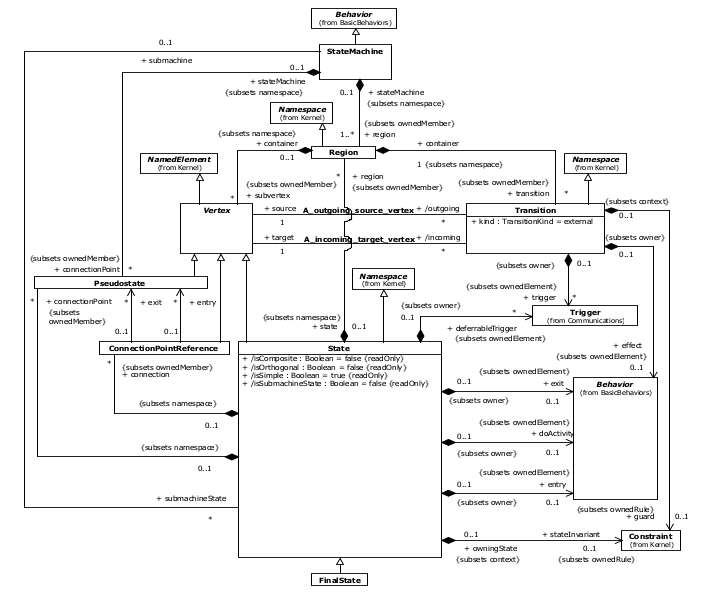
\includegraphics[scale=0.5]{figures/statemachine_metamodel}
\caption{Metamodel of UML state machine}
\label{fig:statemachine_metamodel}
\end{figure}

UML state machines are similar to traditional state machines, but they also have differences. For example UML state charts introduce new features over traditional finite machines such as hierarchically nested regions, orthogonal regions, entry/exit actions, internal transitions and transition execution sequences. The main concepts of this notation are discussed separately.

\begin{description}
	\item[States] are the phases of the system's history. For example if the history can be separated into two phases, then there are two states. 
	\item[Extended states] represents the complete condition of the system. This interpretation means usually states extended with system variables.
	\item[Transitions] happens when a state switched to another.
	\item[Actions] executed when an event dispatched and the system responds by performing them.
	\item[Events] can be everything, that affects the system, and causes state change.
	\item[Guards] are boolean expressions described with extended state variables and event parameters. They can affect the system's behaviour by enabling or disabling transitions.
	\item[Hierarchically nested regions] means that if a system is in a substate then it is also in the same time in all the substate's superstates.
	\item[Orthogonal regions] are regions, which are in 'OR' relation.
	\item[Entry/exit actions] are actions which are dispatched upon entry to a state or exit from it.
	\item[Internal transitions] do not cause state transitions, but only some internal actions to execute and the actual state stays the same.
	\item[Transition execution sequence] describes an execution sequence of actions to do upon event dispatching. First the guard of the transition evaluates. Then the exit actions of the source state configuration will be executed. Then come the actions associated with the transition. Finally the entry actions of the target state configuration will be executed.
\end{description}

% subsubsection umlstatemachine (end)

% subsection modelling (end)

\subsection{Test planning}
\label{sub:testplanning}

Planning tests involves two steps considering the model based test generation process. At first the test selection criteria are chosen, which will be formalised into a test case specification later on.

The main goal of the test selection criteria is to guide the automatic test selection by the test case generation. A good criteria fulfils the previously defined testing policy and testing strategy, that were specified for the system \cite{istqb}. Testing policies give rules for testing, while strategies are high-level guidelines.

Major tasks of test planning consist

\begin{itemize}
	\item determining the scope of the testing and identifying its objectives.
	\item determining the test approach (techniques and coverage).
	\item implementing testing policy and the strategy.
	\item determining the required resources.
	\item scheduling the testing process.
	\item determining exit criteria such as coverage criteria.
\end{itemize}

The required output of the test selection criteria formalisation is the test case specification. This specification have to be fully formalised, so that a test generator is capable of generating test cases based on this formalisation and the software model.

% subsection testplanning (end)

\subsection{Test generation}
\label{sub:testgeneration}

Investigating test case generation algorithms is important, because it has a strong impact on the effectiveness of software testing \cite{testcasegen} \cite{mbttestcasegeneration}. That's why this topic is under activate research and resulted different approaches.

\subsubsection{Adaptive random testing (ART)}
\label{ssub:randomtesting}

Random testing is based on the idea, that the inputs have to spread across the domain of the input parameters to find failure causing inputs. There are five method in the field of ART:

\begin{itemize}
	\item From a randomly generated input set, next candidate is chosen by a selected criterion.
	\item Next input parameter is chosen by exclusion: the randomly generated input parameter has to be outside of previously executed regions (exclusion regions).
	\item One other approach uses the information about previously executed input parameters, to divide the input domain into partitions. Next input parameter will be chosen from a new partition.
	\item The next input parameter can be chosen by dynamically adjusted test profiles.
	\item Distribution metrics can also help to find the next input parameter to achieve dispersion on the input domain.
\end{itemize}

% subsubsection randomtesting (end)

\subsubsection{Search based software testing (SBST)}
\label{ssub:searchbasedtestgen}

In the last few decades there has been an exhausting research in the field of using graph theory at model-based testing. These techniques belong to search-based test generation algorithms.

One of the most used algorithms refers to the \textit{Chinese Postman Problem} \cite{graphtheorymbt}. Given that it is impossible to cross each edge once in an undirected graph during a graph walk, in other words it does not have an Eulerian tour. What is the minimal amount of re-crossing we need to create a walk that uses each edge? The solution is to duplicate the shortest edges between the vertices having odd degree. This process is called "Eulerizing" the graph.

The \textit{New York Street Sweeper Problem} is a variant of the previous graph theory problem. It applies to directed graphs, and arcs need to duplicate to reach, that each nodes have out-degree minus in-degree equal zero. In model-based testing one can use this idea, by creating a transition-based model, which can be represented as a graph. The vertices are the states of the SUT and the edges are the callable methods. A generated Eulerian tour gives a full transition-based structural model coverage.

The previous algorithms give full transition-based coverage, but not pair-wise coverage. The following algorithm named \textit{de Bruijn sequences} creates every combination of the methods. First create a dual graph of the original graph, then eulerize the dual graph (by duplicating arcs to balance node polarities). Create an Eulerian tour, noting the names of the passed nodes.

Dill, Ho, Horowitz and Yang constructed worked on the \textit{limited sub-tour problem} where the test case sequences can not be longer, than a specified upper limit. There is no optimal solution for that problem, but there are some heuristics. For example if an upper limit was set, the current sub-tour has to end and a new sub-tour has to start from that node.

Other approaches using a fitness function to find input parameters that maximises the achievement of test goals, while minimising testing costs.

% subsubsection searchbasedtestgen (end)

\subsubsection{Model checking}
\label{ssub:modelchecking}

This is a traditional model based testing test case generation technique, where a model checker is used to generate test cases. The test criteria are defined as counter examples for the model checker. There are three main approaches in this topic, which are influenced by the chosen modelling notation \cite{sub:modelling}:

\begin{itemize}
	\item \textbf{Axiomatic approaches} Axiomatic foundations of MBT are based on some form of logic calculus. The logic formula has to be transformed into disjunctive normal form (DNF), and this form has to be solved with a higher-order logical theorem prover or the problem has to be transformed into solving finite state machines.
	\item \textbf{Finite state machine approaches} The model is formalised with a Mealy machine, where inputs and outputs are paired on each transition. Test case generation is driven by some test selection criteria.
	\item \textbf{Labelled transition system approaches} This is a common formalism for describing operational semantics of process algebra. There are two common techniques generating test cases (input/output conformance and interface automata), which describe the conformance of the SUT. These techniques do not define test selection strategies, they have to be combined with coverage criteria as seen by FSMs.
\end{itemize}

% subsubsection modelchecking (end)

\subsubsection{Symbolic execution}
\label{ssub:symbolicexecution}

Symbolic execution is a program analysis technique that analyses a program’s code to automatically generate test cases from it. It belongs to white box testing, because the inner structure of the SUT is known during the test.

Symbolic execution uses symbolic values, instead of concrete values, as program inputs. During the symbolic execution the state of the program is represented with \textit{symbolic values} of program variables at that point, a \textit{path constraint} created by symbolic values, and a \textit{program counter}. The path constraint is a Boolean formula, that has to be satisfied to reach that point on the path. At each branch point the path constraint is updated with constraints of the inputs. If the path constraint becomes unsatisfiable, the path can not be continued. If the the path constraint stays satisfiable, then all solution for the Boolean formula can be an input for a given test case.

There are numerous tools which proves the usefulness of this technique, but there are three main problem that limits the effectiveness of this method by real world programs.

\begin{itemize}
	\item \textbf{Path explosion} The most real world program have a huge number of computational path. The execution of each path can be mean an unacceptable overhead. Solutions for this problem can be using the specification of the parts that affect the symbolic execution or avoiding some branch, which are irrelevant to the test data criteria.
	\item \textbf{Path divergence} Programs usually implemented in a mixture of different programming languages. The symbolic execution of such a complex infrastructure is almost impossible. The unavailability of these paths leads to path divergence, and some paths may not be found during the symbolic execution. Possible solution can be to replace these paths with a model during the test generation.
	\item \textbf{Complex constraints} Solving Boolean formulas involves using constraint solvers during the symbolic execution. There are some formula that, which can not be solved with the today available tools. These formulas can be simplified by replacing solvable sub formulas with concrete values.
\end{itemize}

% subsubsection symbolicexecution (end)

\subsubsection{Combinatorial testing}
\label{ssub:combinatorialtesting}

In combinatorial testing samples of input parameters have to be chosen, that cover a prescribed subset of combinations of the elements to be tested. Usually sample consists all t-way combination of possible input parameters, this method is called \textit{combinatorial interaction testing} (CIT). The inputs can be described with a covering array:
\begin{displaymath}
CA=(N;t, k, v),
\end{displaymath}

where $N$ represents sample size, $t$ is called strength, $k$ are the factors and $v$ are the possible symbols. So $CA$ is an $N$ * $k$ array on $v$ symbols such that every $N$ * $t$ sub-array contains all $t$-tuples from the $v$ symbols at least once. Finding an appropriate coverage array is possible using heuristics.

Combinatorial testing can be used if the domains of the input parameters are known.

% subsubsection combinatorialtesting (end)

% subsection testgeneration (end)

\subsection{Test execution}
\label{sub:testexecution}

Test execution includes several steps, because the abstraction level of the generated test cases differ from the SUT. Therefore a previously mentioned adaptor component is needed that bridges between the two component. The concrete execution is done by a component named test script, which includes a test oracle that determines, if the test were run successfully or not.

The tasks of the execution are the followings:

\begin{itemize}
	\item Execute the complete test suite or individual test cases with test scripts.
	\item Log the outcome of the execution and report the identities and versions of the SUT and the testing tools.
	\item Compare the results with the expectations using oracles.
	\item Report the differences between the actual and the expected results.
	\item Repeat the execution with the same configuration to prove the correctness of a previously failed test case. When we just re-execute a test case that called \textit{confirmation testing}, but we have to check that a fix does not introduce new defects (\textit{regression testing}).
\end{itemize}

% subsection testexecution (end)

% section process (end)

% chapter modelbasedtesting (end)